\lab{Introduction to Matplotlib}{Introduction to Matplotlib}
\objective{
Matplotlib is the most commonly used data visualization library in Python. Being able to visualize data helps to determine patterns and communicate results and is a key component of applied and computational mathematics.
In this lab we introduce techniques for visualizing data in 1, 2, and 3 dimensions.
The plotting techniques presented here will be used in the remainder of the labs in the manual.
}

\section*{Line Plots} % =======================================================

Raw numerical data is rarely helpful unless it can be visualized.
The quickest way to visualize a simple 1-dimensional array is with a \emph{line plot}.
The following code creates an array of outputs of the function $f(x) = x^2$, then visualizes the array using the \li{matplotlib} module\footnote{Like NumPy, Matplotlib is \emph{not} part of the Python standard library, but it is included in most Python distributions. See \url{https://matplotlib.org/} for the complete Matplotlib documentation.} \cite{Hunter:2007}.

\begin{lstlisting}
>>> import numpy as np
>>> from matplotlib import pyplot as plt

>>> y = np.arange(-5,6)**2
>>> y
array([25, 16,  9,  4,  1,  0,  1,  4,  9, 16, 25])

# Visualize the plot.
>>> plt.plot(y)                     # Draw the line plot.
<<[<matplotlib.lines.Line2D object at 0x1084762d0>]>>
>>> plt.show()                      # Reveal the resulting plot.
\end{lstlisting}

The result is shown in Figure \ref{fig:basic1}.
Just as \li{np} is a standard alias for NumPy, \li{plt} is a standard alias for \li{matplotlib.pyplot} in the Python community.

The call \li{plt.plot(y)} creates a figure and draws straight lines connecting the entries of \li{y} relative to the $y$-axis.
The $x$-axis is (by default) the index of the array, which in this case is the integers from $0$ to $10$.
Calling \li{plt.show()} then displays the figure.

\begin{figure}[H] % plt.plot(y) compared to plt.plot(x,y).
\captionsetup[subfigure]{justification=centering}
\centering
\begin{subfigure}{.5\textwidth}
    \centering
    \includegraphics[width=\linewidth]{figures/basic1.pdf}
    \caption{\li{plt.plot(y)} uses the indices of\\the array for the $x$-axis.}
    \label{fig:basic1}
\end{subfigure}%
\begin{subfigure}{.5\textwidth}
    \centering
    \includegraphics[width=\linewidth]{figures/basic2.pdf}
    \caption{\li{plt.plot(x,y)} specifies both the\\domain and the range.}
    \label{fig:basic2}
\end{subfigure}
\caption{Plots of $f(x) = x^2$ over the interval $[-5,5]$.}
\end{figure}

\begin{problem} % Law of Large Numbers / NumPy review.
NumPy's \li{random} module has tools for sampling from probability distributions.
For instance, \li{np.random.normal()} draws samples from the normal (Gaussian) distribution.
The \li{size} parameter specifies the shape of the resulting array.
\begin{lstlisting}
>>> np.random.normal(size=(2,3))    # Get a 2x3 array of samples.
array([[ 1.65896515, -0.43236783, -0.99390897],
       [-0.35753688, -0.76738306,  1.29683025]])
\end{lstlisting}
%
Write a function that accepts an integer $n$ as input.
\begin{enumerate}
\item Use \li{np.random.normal()} to create an $n\times n$ array of values randomly sampled from the standard normal distribution.
\item Compute the mean of each row of the array.
\\(Hint: Use \li{np.mean()} and specify the \li{axis} keyword argument.)
\item Return the variance of these means.
\\(Hint: Use \li{np.var()} to calculate the variance).
\end{enumerate}
Define another function that creates an array of the results of the first function with inputs $n = 100,\ 200,\ \ldots,\ 1000$.
Plot (and show) the resulting array.
% This result illustrates one version of the \emph{law of large numbers}.
\end{problem}

\subsection*{Specifying a Domain} % -----------------------------------------

An obvious problem with Figure \ref{fig:basic1} is that the $x$-axis does not correspond correctly to the $y$-axis for the function $f(x) = x^2$ that is being drawn.
To correct this, define an array \li{x} for the domain, then use it to calculate the image \li{y = f(x)}.
The command \li{plt.plot(x,y)} plots \li{x} against \li{y} by drawing a line between the consecutive points \li{(x[i], y[i])}.
% Note that the arrays must have the same number of elements to be compatible.

Another problem with Figure \ref{fig:basic1} is its poor resolution: the curve is visibly bumpy, especially near the bottom of the curve.
NumPy's \li{linspace()} function makes it easy to get a higher-resolution domain.
Recall that \li{np.arange()} returns an array of evenly-spaced values in a given interval, where

% NOTE: the \noindent is to fix a page break problem in PythonEssentials.pdf.

\noindent the \textbf{spacing} between the entries is specified.
In contrast, \li{np.linspace()} creates an array of evenly-spaced values in a given interval where the \textbf{number of elements} is specified.

\begin{lstlisting}
# Get 4 evenly-spaced values between 0 and 32 (including endpoints).
>>> np.linspace(0, 32, 4)
array([  0.        ,  10.66666667,  21.33333333,  32.        ])

# Get 50 evenly-spaced values from -5 to 5 (including endpoints).
>>> x = np.linspace(-5, 5, 50)
>>> y = x**2                        # Calculate the image of f(x) = x**2.
>>> plt.plot(x, y)
>>> plt.show()
\end{lstlisting}

The resulting plot is shown in Figure \ref{fig:basic2}.
This time, the $x$-axis correctly matches up with the $y$-axis.
The resolution is also much better because \li{x} and \li{y} have $50$ entries each instead of only $10$.

Subsequent calls to \li{plt.plot()} modify the same figure until \li{plt.show()} is executed, which displays the current figure and resets the system.
This behavior can be altered by specifying separate figures or axes, which we will discuss shortly.

\begin{info} % Interactive Mode.
Plotting can seem a little mystical because the actual plot doesn't appear until \li{plt.show()} is executed.
Matplotlib's \emph{interactive mode} allows the user to see the plot be constructed one piece at a time.
Use \li{plt.ion()} to turn interactive mode on and \li{plt.ioff()} to turn it off.
This is very useful for quick experimentation.
Try executing the following commands in IPython:

\begin{lstlisting}
<g<In [1]:>g> import numpy as np
<g<In [2]:>g> from matplotlib import pyplot as plt

# Turn interactive mode on and make some plots.
<g<In [3]:>g> plt.ion()
<g<In [4]:>g> x = np.linspace(1, 4, 100)
<g<In [5]:>g> plt.plot(x, np.log(x))
<g<In [6]:>g> plt.plot(x, np.exp(x))

# Clear the figure, then turn interactive mode off.
<g<In [7]:>g> plt.clf()
<g<In [8]:>g> plt.ioff()
\end{lstlisting}

Use interactive mode \textbf{only} with IPython.
Using interactive mode in a non-interactive setting may freeze the window or cause other problems.
\end{info}

\begin{problem} % Plot two lines (sin() and cos()).
Write a function that plots the functions $\sin(x)$, $\cos(x)$, and $\arctan(x)$ on the domain $[-2\pi, 2\pi]$ (use \li{np.pi} for $\pi$).
% Call \li{plt.xlim(-2*np.pi, 2*np.pi)} before \li{plt.show()} to stretch the $x$-axis appropriately.
Make sure the domain is refined enough to produce a figure with good resolution.
\end{problem}

\section*{Plot Customization} % ===============================================

\li{plt.plot()} receives several keyword arguments for customizing the drawing.
For example, the color and style of the line are specified by the following string arguments.
%
\begin{table}[H] % Color and style.
\begin{tabular}{r|l}
    Key & Color \\
    \hline
    \li{'b'} & blue\\
    \li{'g'} & green\\
    \li{'r'} & red\\
    \li{'c'} & cyan\\
    % \li{'m'} & magenta\\
    % \li{'y'} & yellow\\
    \li{'k'} & black\\
    % \li{'w'} & white
\end{tabular}
\qquad
\begin{tabular}{r|l}
    Key & Style \\
    \hline
    \li{'-'} & solid line\\
    \li{'--'} & dashed line\\
    \li{'-.'} & dash-dot line\\
    \li{':'} & dotted line\\
    % \li{'.'} & point marker\\
    \li{'o'} & circle marker\\
    % \li{'*'} & star marker\\
    % \li{'+'} & plus marker
\end{tabular}
\end{table}
%
Specify one or both of these string codes as the third argument to \li{plt.plot()} to change from the default color and style.
Other \li{plt} functions further customize a figure.
%
\begin{table}[H]
\centering
\begin{tabular}{r|l}
    Function & Description\\
    \hline
    % \li{grid()} & Add grid lines\\
    \li{legend()} & Place a legend in the plot\\
    % \li{text()} & Add text at a given position on the plot\\
    \li{title()} & Add a title to the plot\\
    \li{xlim()} / \li{ylim()} & Set the limits of the $x$- or $y$-axis\\
    % \li{xticks()} & set the location of the tick marks on the x axis, returns current locations if no arguments are given\\
    % \li{yticks()} & set the location of the tick marks on the y axis, returns current locations if no arguments are given\\
    \li{xlabel()} / \li{ylabel()} & Add a label to the $x$- or $y$-axis\\
\end{tabular}
\end{table}

\begin{lstlisting}
>>> x1 = np.linspace(-2, 4, 100)
>>> plt.plot(x1, np.exp(x1), 'g:', linewidth=6, label="Exponential")
>>> plt.title("This is the title.", fontsize=18)
>>> plt.legend(loc="upper left")    # plt.legend() uses the 'label' argument of
>>> plt.show()                      # plt.plot() to create a legend.

>>> x2 = np.linspace(1, 4, 100)
>>> plt.plot(x2, np.log(x2), 'r*', markersize=4)
>>> plt.xlim(0, 5)                  # Set the visible limits of the x axis.
>>> plt.xlabel("The x axis")        # Give the x axis a label.
>>> plt.show()
\end{lstlisting}
%
\begin{figure}[H] % Figure customizations.
\captionsetup[subfigure]{justification=centering}
\centering
\begin{subfigure}{.49\textwidth}
    \centering
    \includegraphics[width=\linewidth]{figures/custom1.pdf}
    \label{fig:custom1}
\end{subfigure}
%
\begin{subfigure}{.49\textwidth}
    \centering
    \includegraphics[width=\linewidth]{figures/custom2.pdf}
    \label{fig:custom2}
\end{subfigure}
\label{fig:custom}
\end{figure}

\begin{problem} % Line plots with different domains but uniform style.
Write a function to plot the curve $f(x) = \frac{1}{x-1}$ on the domain $[-2,6]$.
\begin{enumerate}
\item
Although $f(x)$ has a discontinuity at $x=1$, a single call to \li{plt.plot()} in the usual way will make the curve look continuous.
Split up the domain into $[-2,1)$ and $(1,6]$.
Plot the two sides of the curve separately so that the graph looks discontinuous at $x=1$.
\item Plot both curves with a dashed magenta line.
Set the keyword argument \li{linewidth} (or \li{lw}) of \li{plt.plot()} to $4$ to make the line a little thicker than the default setting.
\item Use \li{plt.xlim()} and \li{plt.ylim()} to change the range of the $x$-axis to $[-2,6]$ and the range of the $y$-axis to $[-6, 6]$.
\end{enumerate}
The plot should resemble the figure below.

\begin{figure}[H] % Solution.
\includegraphics[width=.5\textwidth]{figures/discontinuousProblem.pdf}
\end{figure}
\end{problem}

\subsection*{Figures, Axes, and Subplots} % -----------------------------------

The window that \li{plt.show()} reveals is called a \emph{figure}, stored in Python as a \li{plt.Figure} object.
A space on a figure where a plot is drawn is called an \emph{axes}, a \li{plt.Axes} object.
A figure can have multiple axes, and a single program may create several figures.
There are several ways to create or grab figures and axes with \li{plt} functions.

\begin{table}[H]
\centering
\begin{tabular}{r|l}
    Function & Description\\
    \hline
    \li{axes()} & Add an axes to the current figure\\
    \li{figure()} & Create a new figure or grab an existing figure\\
    \li{gca()} & Get the current axes\\
    \li{gcf()} & Get the current figure\\
    \li{subplot()} & Add a single subplot to the current figure\\
    \li{subplots()} & Create a figure and add several subplots to it\\
\end{tabular}
\end{table}

Usually when a figure has multiple axes, they are organized into non-overlapping \emph{subplots}.
The command \li{plt.subplot(nrows, ncols, plot_number)} creates an axes in a subplot grid where \li{nrows} is the number of rows of subplots in the figure, \li{ncols} is the number of columns, and \li{plot_number} specifies which subplot to modify.
If the inputs for \li{plt.subplot()} are all integers, the commas between the entries can be omitted.
For example, \li{plt.subplot(3,2,2)} can be shortened to \li{plt.subplot(322)}.

\begin{figure}[H] % The layout created by subplots(23i).
\captionsetup[subfigure]{justification=centering}
\centering
\begin{framed}
\begin{subfigure}{.32\textwidth}
    \centering
    
\includegraphics[width=\linewidth]{figures/layout_1.pdf}
\end{subfigure}
%
\begin{subfigure}{.32\textwidth}
    \centering
    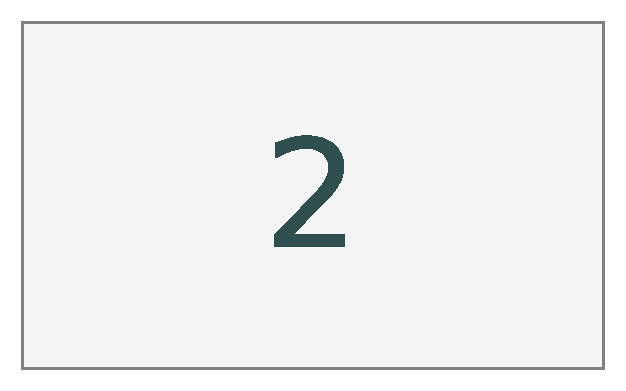
\includegraphics[width=\linewidth]{figures/layout_2.pdf}
\end{subfigure}
%
\begin{subfigure}{.32\textwidth}
    \centering
    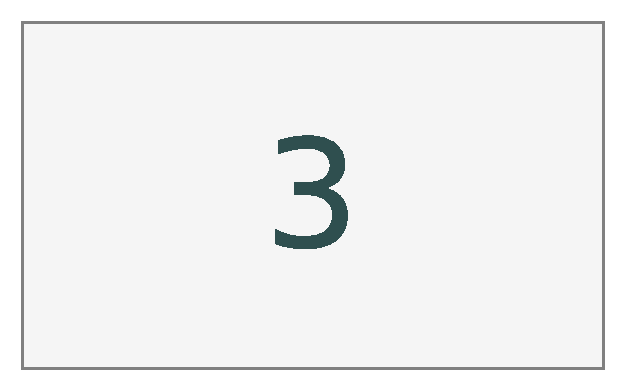
\includegraphics[width=\linewidth]{figures/layout_3.pdf}
\end{subfigure}
\\
\begin{subfigure}{.32\textwidth}
    \centering
    
\includegraphics[width=\linewidth]{figures/layout_4.pdf}
\end{subfigure}
%
\begin{subfigure}{.32\textwidth}
    \centering
    
\includegraphics[width=\linewidth]{figures/layout_5.pdf}
\end{subfigure}
%
\begin{subfigure}{.32\textwidth}
    \centering
    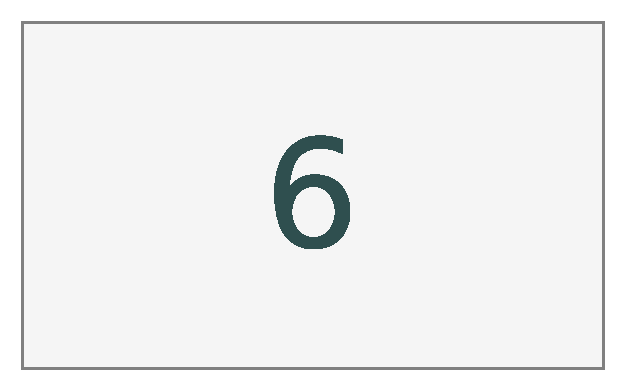
\includegraphics[width=\linewidth]{figures/layout_6.pdf}
\end{subfigure}
\end{framed}
\caption{The layout of subplots with \li{plt.subplot(2,3,i)} (2 rows, 3 columns), where \li{i} is the index pictured above. The outer border is the figure that the axes belong to.}
\label{fig:subplots-layout}
\end{figure}

\begin{lstlisting}
>>> x = np.linspace(.1, 2, 200)
# Create a subplot to cover the left half of the figure.
>>> ax1 = plt.subplot(121)
>>> ax1.plot(x, np.exp(x), 'k', lw=2)
>>> ax1.plot(x, np.exp(2*x), 'b', lw=2)
>>> plt.title("Exponential", fontsize=18)

# Create another subplot to cover the right half of the figure.
>>> ax2 = plt.subplot(122)
>>> ax2.plot(x, np.log(x), 'k', lw=2)
>>> ax2.plot(x, np.log(2*x), 'b', lw=2)
>>> ax2.set_title("Logarithmic", fontsize=18)
>>> plt.show()
\end{lstlisting}

\begin{figure}[H] % The layout created by plt.subplot(23i).
\captionsetup[subfigure]{justification=centering}
\centering
\begin{framed}
\begin{subfigure}{.49\textwidth}
    \centering
    \includegraphics[width=\linewidth]{figures/subplots_1.pdf}
\end{subfigure}
%
\begin{subfigure}{.49\textwidth}
    \centering
    \includegraphics[width=\linewidth]{figures/subplots_2.pdf}
\end{subfigure}
\end{framed}
\end{figure}

\begin{info}
Plotting functions such as \li{plt.plot()} are shortcuts for accessing the current axes on the current figure and calling a method on that \li{Axes} object.
Calling \li{plt.subplot()} changes the current axis, and calling \li{plt.figure()} changes the current figure.
Use \li{plt.gca()} to get the current axes and \li{plt.gcf()} to get the current figure.
Compare the following equivalent strategies for producing a figure with two subplots.

\begin{lstlisting}
>>> x = np.linspace(-5, 5, 100)

# 1. Use plt.subplot() to switch the current.
>>> plt.subplot(121)
>>> plt.plot(x, 2*x)
>>> plt.subplot(122)
>>> plt.plot(x, x**2)

# 2. Use plt.subplot() to explicitly grab the two subplot axes.
>>> ax1 = plt.subplot(121)
>>> ax1.plot(x, 2*x)
>>> ax2 = plt.subplot(122)
>>> ax2.plot(x, x**2)

# 3. Use plt.subplots() to get the figure and all subplots simultaneously.
>>> fig, axes = plt.subplots(1, 2)
>>> axes[0].plot(x, 2*x)
>>> axes[1].plot(x, x**2)
\end{lstlisting}

% Having direct access to the axes and figures as Python objects provides a great deal of flexibility for plot customization.
% If you ever need access to the current axes for detailed customization, use \li{plt.gca()}.
\end{info}

\begin{problem} % Subplots of sine functions.
Write a function that plots the functions $\sin(x)$, $\sin(2x)$, $2\sin(x)$, and $2\sin(2x)$ on the domain $[0, 2\pi]$, each in a separate subplot of a single figure.
\begin{enumerate}
    \item Arrange the plots in a $2\times 2$ grid of subplots.
    \item Set the limits of each subplot to $[0, 2\pi]\times[-2,2]$.
    \\(Hint: Consider using \li{plt.axis([xmin, xmax, ymin, ymax])} instead of \li{plt.xlim()} and \li{plt.ylim()} to set all boundaries simultaneously.)
    \item Use \li{plt.title()} or \li{ax.set_title()} to give each subplot an appropriate title.
    \item Use \li{plt.suptitle()} or \li{fig.suptitle()} to give the overall figure a title.
    \item Use the following colors and line styles.
    \begin{align*}\begin{array}{lcl}
    \sin(x)\text{: green solid line.} && \sin(2x)\text{: red dashed line.}\\ \\
    2\sin(x)\text{: blue dashed line.} && 2\sin(2x)\text{: magenta dotted line.}
    \end{array}\end{align*}
\end{enumerate}
\end{problem}

\begin{warn}
Be careful not to mix up the following functions.
\begin{enumerate}
    \item \li{plt.axes()} creates a new place to draw on the figure, while \li{plt.axis()} (or \li{ax.axis()}) sets properties of the $x$- and $y$-axis in the current axes, such as the $x$ and $y$ limits.
    \item \li{plt.subplot()} (singular) returns a single subplot belonging to the current figure, while \li{plt.subplots()} (plural) creates a new figure and adds a collection of subplots to it.
\end{enumerate}
% The \li{subplots()} function is especially useful for figures with many subplots.
% \begin{lstlisting}
% # The subplot axes are organized in an array of the given shape.
% >>> fig, ax = plt.sublplots(2,3)
% >>> ax.shape
% (2, 3)
% >>> ax[1,1].plot([1,2,3],[4,5,6])
% # ...
% \end{lstlisting}
\end{warn}

\section*{Other Kinds of Plots} % =============================================

Line plots are not always the most illuminating choice of graph to describe a set of data.
Matplotlib provides several other easy ways to visualize data.

\begin{itemize}
\item A \emph{scatter plot} plots two 1-dimensional arrays against each other without drawing lines between the points.
Scatter plots are particularly useful for data that is not correlated or ordered.

To create a scatter plot, use \li{plt.plot()} and specify a point marker (such as \li{'o'} or \li{'*'}) for the line style, or use \li{plt.scatter()} (or \li{ax.scatter()}).
Beware that \li{plt.scatter()} has slightly different arguments and syntax than \li{plt.plot()}.

\item A \emph{histogram} groups entries of a 1-dimensional data set into a given number of intervals, called \emph{bins}.
Each bin has a bar whose height indicates the number of values that fall in the range of the bin.
% The more bins, the greater the detail, but having too many bins can also destroy the picture by creating interval gaps between values.
Histograms are best for displaying distributions, relating data values to frequency.

To create a histogram, use \li{plt.hist()} (or \li{ax.hist()}).
Use the argument \li{bins} to specify the edges of the bins or to choose a number of bins.
The \li{<<range>>} argument specifies the outer limits of the first and last bins.
\end{itemize}

\begin{lstlisting}
# Get 500 random samples from two normal distributions.
>>> x = np.random.normal(scale=1.5, size=500)
>>> y = np.random.normal(scale=0.5, size=500)

# Draw a scatter plot of x against y, using transparent circle markers.
>>> ax1 = plt.subplot(121)
>>> ax1.plot(x, y, 'o', markersize=5, alpha=.5)

# Draw a histogram to display the distribution of the data in x.
>>> ax2 = plt.subplot(122)
>>> ax2.hist(x, bins=np.arange(-4.5, 5.5))      # Or, equivalently,
#   ax2.hist(x, bins=9, range=[-4.5, 4.5])

>>> plt.show()
\end{lstlisting}

\begin{figure}[H]
\captionsetup[subfigure]{justification=centering}
\centering
\begin{framed}
\begin{subfigure}{.49\textwidth}
    \centering
    \includegraphics[width=\linewidth]{figures/scatterplot.pdf}
\end{subfigure}
%
\begin{subfigure}{.49\textwidth}
    \centering
    \includegraphics[width=\linewidth]{figures/histogram.pdf}
\end{subfigure}
\end{framed}
\end{figure}

% On the histogram, specifying 9 bins in the range $[-4.5, 4.5]$ creates a bin centered over each integer from $-4$ to $4$.

\begin{problem} % FARS data visualization.
The Fatality Analysis Reporting System (FARS) is a nationwide census that provides yearly data regarding fatal injuries suffered in motor vehicle traffic crashes.%
\footnote{See \url{http://www.nhtsa.gov/FARS}.}
The array contained in \texttt{FARS.npy} is a small subset of the FARS database from 2010--2014.
Each of the 148,206 rows in the array represents a different car crash; the columns represent the hour (in military time, as an integer), the longitude, and the latitude, in that order.

Write a function to visualize the data in \texttt{FARS.npy}.
Use \li{np.load()} to load the data, then create a single figure with two subplots:
%
\begin{enumerate}
\item A scatter plot of longitudes against latitudes.
Because of the large number of data points, use black pixel markers (use \li{"k,"} as the third argument to \li{plt.plot()}).
Label both axes using \li{plt.xlabel()} and \li{plt.ylabel()} (or \li{ax.set_xlabel()} and \li{ax.set_ylabel()}).
\\
(Hint: Use \li{plt.axis("equal")} or \li{ax.set_aspect("equal")} so that the $x$- and $y$-axis are scaled the same way.

\item A histogram of the hours of the day, with one bin per hour.
Set the limits of the $x$-axis appropriately.
Label the $x$-axis.
You should be able to clearly see which hours of the day experience more traffic.
\end{enumerate}
\end{problem}

Matplotlib also has tools for creating other kinds of plots for visualizing 1-dimensional data, including bar plots and box plots.
See the Matplotlib Appendix for examples and syntax.

\subsection*{Visualizing 3-D Surfaces} % --------------------------------------

Line plots, histograms, and scatter plots are good for visualizing $1$- and $2$-dimensional data, including the domain and range of a function $f:\mathbb{R}\rightarrow\mathbb{R}$.
However, visualizing $3$-dimensional data or a function $g:\mathbb{R}^2\rightarrow\mathbb{R}$ (two inputs, one output) requires a different kind of plot.
The process is similar to creating a line plot but requires slightly more setup: first construct an appropriate domain, then calculate the image of the function on that domain.

NumPy's \li{np.meshgrid()} function is the standard tool for creating a 2-dimensional domain in the Cartesian plane.
Given two 1-dimensional coordinate arrays, \li{np.meshgrid()} creates two corresponding coordinate matrices.
See Figure \ref{fig:meshgrid}.

\begin{figure}[H] % np.meshgrid() visual demonstration.
%\begin{tikzpicture}[>=stealth', shorten <= .1cm,shorten >=.1cm, dot/.style=
%    {circle,fill=black,minimum size=3pt,inner sep=0pt, outer sep=-1pt} ]
%
%\foreach \x/\y in {0/0, 0/2, 0/4, 2/0, 2/2, 2/4, 4/0, 4/2, 4/4}
%    \node[draw, dot]at(\x,\y){};
%\foreach \x/\y in {0/0, 0/1, 0/2, 1/0, 1/1, 1/2, 2/0, 2/1, 2/2}
%    \node[draw=none]at(\x*2-.5, \y*2+.3){(\x,\y)};
%
%\foreach \x/\y in {0/0, 0/1, 0/2, 1/0, 1/1, 1/2, 2/0, 2/1, 2/2}
%    \node[draw=none]at(\x*.75+7, \y*.75+.1){\y};
%\foreach \x/\y in {0/0, 0/1, 0/2, 1/0, 1/1, 1/2, 2/0, 2/1, 2/2}
%    \node[draw=none]at(\x*.75+7, \y*-.75+3.9){\x};
%
%\draw[-, thick](6.7,-.25)--(6.7,1.95);
%\draw[-, thick](8.8,-.25)--(8.8,1.95);
%\draw[-, thick](6.7,2.05)--(6.7,4.25);
%\draw[-, thick](8.8,2.05)--(8.8,4.25);
%\draw[-, thick](8.8,4.14)--(8.7,4.14);
%\draw[-, thick](8.8,2.16)--(8.7,2.16);
%\draw[-, thick](6.7,4.14)--(6.8,4.14);
%\draw[-, thick](6.7,2.16)--(6.8,2.16);
%\draw[-, thick](8.8,1.84)--(8.7,1.84);
%\draw[-, thick](8.8,-.135)--(8.7,-.135);
%\draw[-, thick](6.8,1.84)--(6.7,1.84);
%\draw[-, thick](6.8,-.135)--(6.7,-.135);
%
%\node[draw=none](X)at(6.3,.9){\texttt{Y}=};
%\node[draw=none](y)at(6.3,3.15){\texttt{X}=};
%
%\node[draw=none](point1)at(-.3, -.6){\texttt{x}=\big[0,};
%\node[draw=none, node distance=2.35cm](point2)
%    [right of=point1]{1,};
%\node[draw=none, node distance=2cm](point3)
%    [right of=point2]{2\big]};
%\node[draw=none, rotate=270](point4)at(4.6,4.25)
%    {\texttt{y}=\big[2,};
%\node[draw=none, rotate=270, node distance=2.35cm](point5)
%    [right of=point4]{1,};
%\node[draw=none, rotate=270, node distance=2cm](point6)
%    [right of=point5]{0\big]};
%\end{tikzpicture}

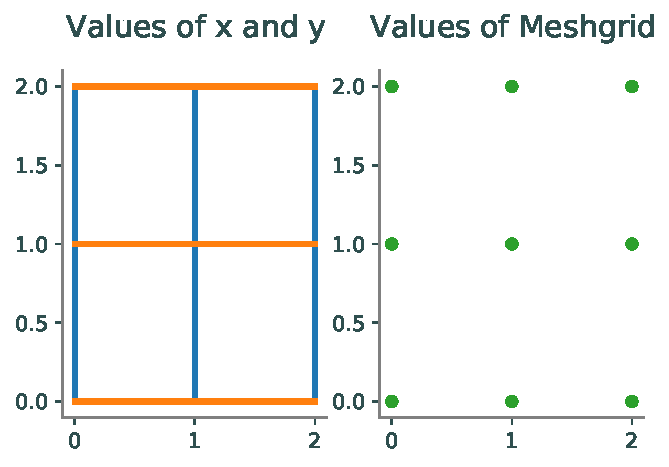
\includegraphics[width=\linewidth]{figures/meshplot_fig.pdf}

\caption[Meshplot example]{In the left plot, we have two arrays where x and y have the values \texttt{x = y = [0,1,2]}. The command \texttt{np.meshgrid(x, y)} returns the arrays 
$X= \begin{bmatrix} 0 & 1 & 2 \\

 0 & 1 & 2 \\
 0 & 1 & 2 \end{bmatrix}$ and $Y= \begin{bmatrix} 0 & 0 & 0 \\
 1 & 1 & 1 \\
 2 & 2 & 2\end{bmatrix}.$

 These give the $x$- and $y$-coordinates of the points in the grid formed by \texttt{x} and \texttt{y} as seen in the right plot and satisfy the relation \texttt{(X[i,j], Y[i,j]) = (x[j],y[i])}.}

\label{fig:meshgrid}
\end{figure}

\begin{lstlisting}
>>> x, y = [0, 1, 2], [3, 4, 5]     # A rough domain over [0,2]x[3,5].
>>> X, Y = np.meshgrid(x, y)        # Combine the 1-D data into 2-D data.
>>> for xrow, yrow in zip(X,Y):
...     print(xrow, yrow, sep='\t')
...
[0 1 2]    [3 3 3]
[0 1 2]    [4 4 4]
[0 1 2]    [5 5 5]
\end{lstlisting}

With a 2-dimensional domain, $g(x,y)$ is usually visualized with two kinds of plots.

\begin{itemize}
\item A \emph{heat map} assigns a color to each point in the domain, producing a 2-dimensional colored picture describing a 3-dimensional shape.
Darker colors typically correspond to lower values while lighter colors typically correspond to higher values.

Use \li{plt.pcolormesh()} to create a heat map. You can add an optional argument for the shading type; this determines the layout and fill style of the heat map. This argument defaults to \li{shading='auto'}, and will automatically choose a fill method suited to the data being graphed.

\item A \emph{contour map} draws several \emph{level curves} of $g$ on the $2$-dimensional domain.
A level curve corresponding to the constant $c$ is the collection of points $\left\{(x,y)\mid c = g(x,y)\right\}$.
Coloring the space between the level curves produces a discretized version of a heat map.
Including more and more level curves makes a filled contour plot look more and more like the complete, blended heat map.

Use \li{plt.contour()} to create a contour plot and \li{plt.contourf()} to create a filled contour plot.
Specify either the number of level curves to draw, or a list of constants corresponding to specific level curves.
\end{itemize}

These functions each receive the keyword argument \li{cmap} to specify a color scheme (some of the better schemes are \li{"viridis"}, \li{"magma"}, and \li{"coolwarm"}).
For the list of all Matplotlib color schemes, see \url{http://matplotlib.org/examples/color/colormaps_reference.html}.

Finally, \li{plt.colorbar()} draws the color scale beside the plot to indicate how the colors relate to the values of the function.

\begin{lstlisting}
# Create a 2-D domain with np.meshgrid().
>>> x = np.linspace(-np.pi, np.pi, 100)
>>> y = x.copy()
>>> X, Y = np.meshgrid(x, y)
>>> Z = np.sin(X) * np.sin(Y)       # Calculate g(x,y) = sin(x)sin(y).

# Plot the heat map of f over the 2-D domain.
>>> plt.subplot(131)
>>> plt.pcolormesh(X, Y, Z, cmap="viridis", shading="auto")
>>> plt.colorbar()
>>> plt.xlim(-np.pi, np.pi)
>>> plt.ylim(-np.pi, np.pi)

# Plot a contour map of f with 10 level curves.
>>> plt.subplot(132)
>>> plt.contour(X, Y, Z, 10, cmap="coolwarm")
>>> plt.colorbar()

# Plot a filled contour map, specifying the level curves.
>>> plt.subplot(133)
>>> plt.contourf(X, Y, Z, [-1, -.8, -.5, 0, .5, .8, 1], cmap="magma")
>>> plt.colorbar()
>>> plt.show()
\end{lstlisting}

\begin{figure}[H] % heat map and contour plots.
\captionsetup[subfigure]{justification=centering}
\centering
\begin{framed}
\begin{subfigure}{.33\textwidth}
    \centering
    \includegraphics[width=\linewidth]{figures/heatmap.png}
\end{subfigure}%
\begin{subfigure}{.33\textwidth}
    \centering
    \includegraphics[width=\linewidth]{figures/contour.pdf}
\end{subfigure}%
\begin{subfigure}{.33\textwidth}
    \centering
    \includegraphics[width=\linewidth]{figures/contourf.pdf}
\end{subfigure}
\end{framed}
\end{figure}

\begin{problem} % Heat map / contour plot of a function f:R2->R.
\label{prob:heatmap}
Write a function to plot $g(x,y) = \frac{\sin(x)\sin(y)}{xy}$ on the domain $[-2\pi,2\pi] \times [-2\pi,2\pi]$.

\begin{enumerate}
\item Create 2 subplots: one with a heat map of $g$, and one with a contour map of $g$.
Choose an appropriate number of level curves, or specify the curves yourself.
\item Set the limits of each subplot to $[-2\pi,2\pi] \times [-2\pi,2\pi]$.
\item Choose a non-default color scheme.
\item Include a color scale bar for each subplot.
\end{enumerate}
\end{problem}

\begin{comment}
\begin{info} % Note about plt.imshow().
Black-and-white pictures are usually stored as a $2$-dimensional array and colord pictures are stored as a $3$-dimensional array (a stack of 2-dimensional arrays, one for each RGB value).
This kind of data does not require a domain, and is easily visualized with \li{plt.imshow()}.
\end{info}
\end{comment}

\newpage

\section*{Additional Material} % ==============================================

\subsection*{Further Reading and Tutorials} % ---------------------------------

Plotting takes some getting used to.
See the following materials for more examples.
\begin{itemize}
    \item \url{https://www.labri.fr/perso/nrougier/teaching/matplotlib/}.
    \item \url{https://matplotlib.org/stable/tutorials/introductory/pyplot.html}.
    \item \url{http://scipy-lectures.org/intro/matplotlib/}.
    \item The Matplotlib Appendix in this manual.
\end{itemize}

\subsection*{3-D Plotting} % --------------------------------------------------

Matplotlib can also be used to plot 3-dimensional surfaces.
The following code produces the surface corresponding to $g(x,y) = \sin(x)\sin(y)$.

\begin{lstlisting}
# Create the domain and calculate the range like usual.
>>> x = np.linspace(-np.pi, np.pi, 200)
>>> y = np.copy(x)
>>> X, Y = np.meshgrid(x, y)
>>> Z = np.sin(X) * np.sin(Y)

# Draw the corresponding 3-D plot using some extra tools.
>>> fig = plt.figure()
>>> ax = fig.add_subplot(1,1,1, projection='3d')
>>> ax.plot_surface(X, Y, Z)
>>> plt.show()
\end{lstlisting}

\begin{figure}[H]
    \includegraphics[width=.7\textwidth]{figures/surface_plot.pdf}
\end{figure}

\subsection*{Animations} % ----------------------------------------------------

Lines and other graphs can be altered dynamically to produce animations.
Follow these steps to create a Matplotlib animation:
%
\begin{enumerate}
    \item Calculate all data that is needed for the animation.
    \item Define a figure explicitly with \li{plt.figure()} and set its window boundaries.
    \item Draw empty objects that can be altered dynamically.
    \item Define a function to update the drawing objects.
    \item Use \li{matplotlib.animation.FuncAnimation()}.
\end{enumerate}

The submodule \li{matplotlib.animation} contains the tools for putting together and managing animations.
The function \li{matplotlib.animation.FuncAnimation()} accepts the figure to animate, the function that updates the figure, the number of frames to show before repeating, and how fast to run the animation (lower numbers mean faster animations).

\begin{lstlisting}
from matplotlib.animation import FuncAnimation

def sine_animation():
    # Calculate the data to be animated.
    x = np.linspace(0, 2*np.pi, 200)[:-1]
    y = np.sin(x)

    # Create a figure and set the window boundaries of the axes.
    fig = plt.figure()
    plt.xlim(0, 2*np.pi)
    plt.ylim(-1.2, 1.2)

    # Draw an empty line. The comma after 'drawing' is crucial.
    drawing, = plt.plot([],[])

    # Define a function that updates the line data.
    def update(index):
        drawing.set_data(x[:index], y[:index])
        return drawing,                     # Note the comma!

    a = FuncAnimation(fig, update, frames=len(x), interval=10)
    plt.show()
\end{lstlisting}

Try using the following function in place of \li{update()}.
Can you explain why this animation is different from the original?

\begin{lstlisting}
def wave(index):
    drawing.set_data(x, np.roll(y, index))
    return drawing,
\end{lstlisting}

% \begin{comment} % Too much.
To animate multiple objects at once, define the objects separately and make sure the update function returns both objects.

\begin{lstlisting}
def sine_cosine_animation():
    x = np.linspace(0, 2*np.pi, 200)[:-1]
    y1, y2 = np.sin(x), np.cos(x)

    fig = plt.figure()
    plt.xlim(0, 2*np.pi)
    plt.ylim(-1.2, 1.2)

    sin_drawing, = plt.plot([],[])
    cos_drawing, = plt.plot([],[])

    def update(index):
        sin_drawing.set_data(x[:index], y1[:index])
        cos_drawing.set_data(x[:index], y2[:index])
        return sin_drawing, cos_drawing,

    a = FuncAnimation(fig, update, frames=len(x), interval=10)
    plt.show()
\end{lstlisting}
% \end{comment}

\begin{comment} % Too much.
Animations are very useful for describing parametrized curves, as the ``speed'' of the curve is displayed.
The code below animates the rose curve, parametrized by the angle $\theta \in [0, 2\pi]$, given by the following equations.
%
\[\begin{array}{ccc}
x(\theta) = \cos(\theta)\cos(6\theta), && y(\theta) = \sin(\theta)\cos(6\theta)
\end{array}\]

\begin{lstlisting}
def rose_animation():
    # Calculate the parametrized data.
    theta = np.linspace(0, 2*np.pi, 200)
    x = np.cos(theta)*np.cos(6*theta)
    y = np.sin(theta)*np.cos(6*theta)

    fig = plt.figure()
    plt.xlim(-1.2, 1.2)
    plt.ylim(-1.2, 1.2)
    plt.gca().set_aspect("equal")           # Make the figure exactly square.

    drawing, = plt.plot([],[])

    # Define a function that updates the line data.
    def update(index):
        drawing.set_data(x[:index], y[:index])
        return drawing,

    a = FuncAnimation(fig, update, frames=len(x), interval=10, repeat=False)
    plt.show()              # repeat=False freezes the animation at the end.
\end{lstlisting}
\end{comment}

Animations can also be 3-dimensional.
The only major difference is an extra operation to set the 3-dimensional component of the drawn object.
The code below animates the space curve parametrized by the following equations:
%
\[\begin{array}{ccccc}
x(\theta) = \cos(\theta)\cos(6\theta), &&
y(\theta) = \sin(\theta)\cos(6\theta), &&
z(\theta) = \frac{\theta}{10}
\end{array}\]

\begin{lstlisting}
def rose_animation_3D():
    theta = np.linspace(0, 2*np.pi, 200)
    x = np.cos(theta) * np.cos(6*theta)
    y = np.sin(theta) * np.cos(6*theta)
    z = theta / 10

    fig = plt.figure()
    ax = fig.add_subplot(projection='3d')           # Make the figure 3-D.
    ax.set_xlim3d(-1.2, 1.2)                # Use ax instead of plt.
    ax.set_ylim3d(-1.2, 1.2)
    ax.set_aspect("equal")

    drawing, = ax.plot([],[],[])            # Provide 3 empty lists.

    # Update the first 2 dimensions like usual, then update the 3-D component.
    def update(index):
        drawing.set_data(x[:index], y[:index])
        drawing.set_3d_properties(z[:index])
        return drawing,

    a = FuncAnimation(fig, update, frames=len(x), interval=10, repeat=False)
    plt.show()
\end{lstlisting}

% See \url{https://matplotlib.org/2.0.0/examples/animation/index.html} for more examples.

\begin{comment} % TODO: An ORIGINAL example of using widgets
\subsection*{Interactive Plots} % ---------------------------------------------

Matplotlib plots can be made interactive by adding \emph{widgets}.
Consider the following example, TAKEN FROM THE MATPLOTLIB DOCS BASICALLY AHHH

\begin{lstlisting}
>>> from matplotlib import widgets as wg

>>> ax = plt.subplot(111)
>>> plt.subplots_adjust(bottom=.25)         # Make some space for a slider bar.
>>> t = np.arange(0., 1., .001)
>>> a0 = 5.
>>> f0 = 3.
>>> s = a0 * np.sin(2 * np.pi * f0 * t)
>>> l = plt.plot(t, s)[0]
>>> plt.axis([0, 1, -10, 10])
>>> axfreq = plt.axes([.25, .05, .65, .03])
>>> axamp = plt.axes([.25, .1, .65, .03])

# Make some slider bars.
>>> sfreq = wg.Slider(axfreq, 'Freq', .1, 30., valinit=f0)
>>> samp = wg.Slider(axamp, 'Amp', .1, 10., valinit=a0)
>>> def update(val):                        # Function for updating the plot.
...     amp = samp.val                          # Read from one slider.
...     freq = sfreq.val                        # Read from the other slider.
...     l.set_ydata(amp * np.sin(2 * np.pi * freq * t))
...     plt.draw()                              # Refresh the plot.
>>> sfreq.on_changed(update)                # Connect the sliders to update().
>>> samp.on_changed(update)
>>> plt.show()
\end{lstlisting}

\begin{figure}[H]
\includegraphics[width=.7\textwidth]{figures/interactive_plot.pdf}
\end{figure}
\end{comment}

% =============================================================================
% =============================================================================
% Stuff to move ===============================================================
% =============================================================================
% =============================================================================

\begin{comment}
\begin{info} % IPython Notebook inline plotting (move to notebook intro)
If you are executing these Matplotlib commands in an IPython shell, executing the \li{plt.show()} method will open a new window with the plot.
If you are using IPython Notebook, you have the option to display the plots within your notebook.
You may opt into this feature by running \li{\%matplotlib inline} or \li{\%matplotlib notebook} in your IPython Notebook.
The \li{inline} option shows the plot, whereas the \li{notebook} option shows the plot and provides controls to interact with the plot.
Additionally, when using this option, the plot is displayed after running the \li{plt.plot()} command; the \li{plt.show()} command is not necessary.
\end{info}
\end{comment}
